%Version 3.1 December 2024
% See section 11 of the User Manual for version history
%
%%%%%%%%%%%%%%%%%%%%%%%%%%%%%%%%%%%%%%%%%%%%%%%%%%%%%%%%%%%%%%%%%%%%%%
%%                                                                 %%
%% Please do not use \input{...} to include other tex files.       %%
%% Submit your LaTeX manuscript as one .tex document.              %%
%%                                                                 %%
%% All additional figures and files should be attached             %%
%% separately and not embedded in the \TeX\ document itself.       %%
%%                                                                 %%
%%%%%%%%%%%%%%%%%%%%%%%%%%%%%%%%%%%%%%%%%%%%%%%%%%%%%%%%%%%%%%%%%%%%%

\documentclass[pdflatex,sn-mathphys-num]{sn-jnl}% Math and Physical Sciences Numbered Reference Style

%%%% Standard Packages
\usepackage{graphicx}%
\usepackage{multirow}%
\usepackage{amsmath,amssymb,amsfonts}%
\usepackage{amsthm}%
\usepackage{mathrsfs}%
\usepackage[title]{appendix}%
\usepackage{xcolor}%
\usepackage{textcomp}%
\usepackage{manyfoot}%
\usepackage{booktabs}%
\usepackage{algorithm}%
\usepackage{algorithmicx}%
\usepackage{algpseudocode}%
\usepackage{listings}%
%%%%


\theoremstyle{thmstyleone}%
\newtheorem{theorem}{Theorem}%
\newtheorem{proposition}[theorem]{Proposition}%
\theoremstyle{thmstyletwo}%
\newtheorem{example}{Example}%
\newtheorem{remark}{Remark}%
\theoremstyle{thmstylethree}%
\newtheorem{definition}{Definition}%

\raggedbottom

\begin{document}

\title[Leakage-free, imbalance-aware evaluation of phishing URL classifiers]{Beyond Benchmark Accuracy: Leakage-Free and Imbalance-Aware Evaluation of Fine-Tuned Phishing URL Classifiers}

%% One \author line per team member; the corresponding author uses \author* and \affil*.
\author*[1]{\fnm{Neha} \sur{Tirkey}}\email{neha.tirkey.ug24@nsut.ac.in}

\affil*[1]{\orgdiv{Department of Information Technology (Network and Information Security)}, \orgname{Netaji Subhas University of Technology}, \orgaddress{\city{New Delhi}, \postcode{110078}, \state{Delhi}, \country{India}}}

\abstract{Machine learning detectors of phishing URLs routinely report 97--98\% accuracy on public benchmark datasets. This study tests whether such figures survive stricter evaluation, taking as its reference a recent SCIE-indexed study that tuned eight classifiers with SMOTE balancing, grid search and feature selection. Three experiments were run. Replicating the eight classifiers showed that balancing the whole dataset before cross-validation, as the reference study did, raised accuracy on the UCI dataset for every classifier, by 0.25 to 2.73 percentage points, compared with leakage-free nested cross-validation; the already balanced Mendeley dataset showed no such gap. On the 2024 PhiUSIIL dataset of 235,795 URLs, the precision of classifiers using URL-only features fell from at least 99.2\% on balanced test sets to between 54.9\% and 99.2\% when legitimate URLs outnumbered phishing URLs 100 to 1, within 0.5 points of an analytic prediction, while accuracy rose. All models predicted in under 70 $\mu$s per URL, but a single supplied PhiUSIIL feature separates the classes with 99.66\% accuracy and every legitimate URL is a bare home page, which explains its near-perfect scores. Studies should therefore report leakage-free estimates, false-positive rates and precision at realistic class ratios.}

\keywords{Phishing detection, Malicious URL, Machine learning, Data leakage, Class imbalance, Hyper-parameter tuning}

\maketitle

%%=====================================================================%%
\section{Introduction}\label{sec1}

Phishing is one of the most widespread forms of cybercrime. An attacker imitates a trusted organisation and persuades the victim to open a link to a fraudulent website, where passwords, payment details or other personal data are collected, or malware is installed. Citing figures from the Anti-Phishing Working Group, Abdul Samad et al.\ \cite{abdulsamad2023} report that more than one million phishing attacks were recorded in the first quarter of 2022 alone, the highest quarterly total reported up to that point. At this scale, protection cannot rely on users recognising fraudulent pages, and the automatic detection of malicious URLs has become an active research area \cite{sahoo2017,tang2021,safi2023}.

The simplest defences compare a URL with a blacklist of known phishing addresses or a whitelist of trusted ones. They are fast, but they cannot recognise a phishing URL that has not yet been reported. Heuristic methods generalise better by applying rules derived from known attacks, but the rules must be designed and maintained by experts \cite{tang2021,abdulsamad2023}. Machine learning methods instead learn the decision rule from labelled examples. They describe each website with lexical features of the URL string, content features of the page's HTML and JavaScript, and external features such as domain age, DNS records, search-engine indexing or traffic rank \cite{sahoo2017,tang2021}. A systematic review of 80 recent studies found that machine learning was the most frequently applied family of techniques (57 studies) and random forest the most frequently used classifier (31 studies) \cite{safi2023}.

On the two public benchmark datasets used most often, the UCI Phishing Websites dataset \cite{mohammad2012uci} and the Mendeley phishing dataset \cite{tan2018}, reported accuracies now lie between about 97\% and 98.6\% \cite{khan2020,salihovic2019,alsarem2021,abdulsamad2023}. A recent SCIE-indexed study by Abdul Samad et al.\ \cite{abdulsamad2023} showed that combining three tuning factors (data balancing with SMOTE, hyper-parameter tuning and feature selection) raises eight standard classifiers to 97.47\% accuracy on the UCI dataset and 98.27\% on the Mendeley dataset. Three aspects of how such figures are obtained, however, limit what they say about a detector in use. First, the study normalises and balances the whole dataset before it is split, so synthetic samples created from test rows can enter the training data, and tuning decisions are made on the same folds that are reported \cite{varma2006}. Second, both benchmarks are close to balanced, whereas legitimate URLs far outnumber phishing URLs in real traffic. Fig.~\ref{fig:motivation} applies the study's own reported precision and recall to this situation: the precision of its best tuned model would fall from 98.5\% to about 40\% if legitimate URLs outnumbered phishing URLs 100 to 1. Third, accuracy is reported without the computational cost of training and prediction, and without the cost of features that require downloading the page or querying external services.

\begin{figure}[htbp]
\centering
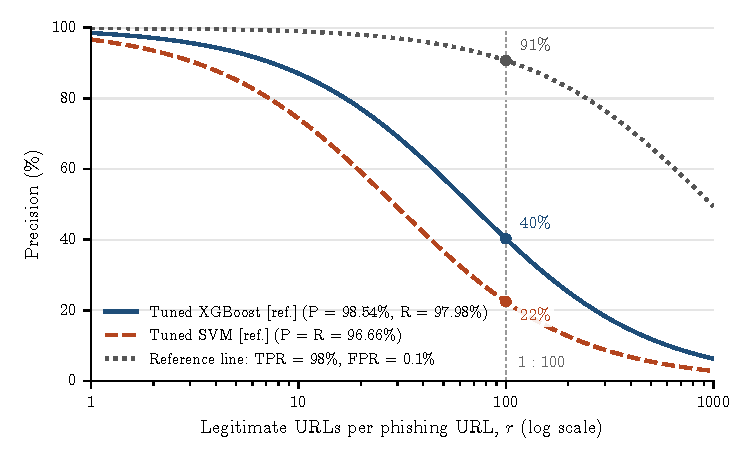
\includegraphics[width=0.9\textwidth]{fig_motivation.pdf}
\caption{Precision expected when legitimate URLs outnumber phishing URLs $r$ to 1, computed with Eqs.~(\ref{eq:prec-ratio}) and (\ref{eq:fpr-balanced}) from the precision and recall that Abdul Samad et al.\ \cite{abdulsamad2023} report for tuned XGBoost and SVM on the balanced Mendeley dataset. The dotted reference curve shows the error rates a detector would need to keep precision above 90\% at $r=100$}\label{fig:motivation}
\end{figure}

This paper tests these three issues experimentally. Its main contributions are as follows:
\begin{itemize}
\item A replication of the eight fine-tuned classifiers of Abdul Samad et al.\ \cite{abdulsamad2023} on both benchmark datasets, under the original preprocessing protocol and under leakage-free nested cross-validation, which measures how much of the reported accuracy depends on the protocol (experiment E1).
\item A class-imbalance stress test on PhiUSIIL \cite{prasad2024}, a dataset of 235,795 URLs published in 2024, which measures precision, recall, the Matthews correlation coefficient (MCC) and the area under the precision--recall curve (PR-AUC) at 1, 10 and 100 legitimate URLs per phishing URL, and compares the observed precision with an analytic prediction (experiment E2).
\item A cost analysis that compares the 50 numeric features supplied with PhiUSIIL against 23 lexical features computed from the URL string alone, in terms of training time, prediction time and detection quality (experiment E3).
\item An open-source implementation that reproduces every table and figure in this paper with a single command.
\end{itemize}

The source code, raw results and figures are available at \url{https://github.com/nehatirkey-nsut/phishing-url-evaluation}. The rest of the paper is organised as follows. Section~\ref{sec2} reviews related work and states the research gap. Section~\ref{sec3} presents the research questions, the architecture of the evaluation framework, the datasets, features, algorithms and metrics. Section~\ref{sec4} describes the implementation and experimental setup, Section~\ref{sec5} reports the results and compares them with earlier work, Section~\ref{sec6} discusses their implications and limitations, and Section~\ref{sec7} concludes.

%%=====================================================================%%
\section{Literature Review}\label{sec2}

\subsection{Approaches to phishing URL detection}\label{subsec2-1}

Sahoo et al.\ \cite{sahoo2017} frame malicious URL detection as a binary classification problem and organise the literature by feature representation (lexical, host-based and content-based) and by learning algorithm. Tang and Mahmoud \cite{tang2021} follow the life cycle of a phishing attack, review common anti-phishing methods, and examine machine learning solutions step by step, from data collection and feature extraction to modelling and performance evaluation. Safi and Singh \cite{safi2023} systematically review 80 studies published over five years and compare list-based, visual-similarity, heuristic, machine learning and deep learning techniques. They report that PhishTank was the main source of phishing URLs (53 studies) and Alexa rankings the main source of legitimate ones (29 studies), and that the highest accuracy reported, 99.98\%, was obtained by a convolutional neural network.

Recent systems differ mainly in how URLs are represented and where the model runs. Ahammad et al.\ \cite{ahammad2022} applied several machine learning methods to phishing URL detection, and Abdul Samad et al.\ \cite{abdulsamad2023} studied how data balancing, hyper-parameter tuning and feature selection change the accuracy of eight standard classifiers. Alani and Tawfik \cite{alani2022} proposed PhishNot, a cloud-based machine learning approach aimed at practical deployment. Representation-learning methods avoid hand-crafted features altogether: URLNet \cite{le2018} learns character-level and word-level representations of the URL with convolutional neural networks, and Elsadig et al.\ \cite{elsadig2022} extracted features from URL text with the BERT language model \cite{devlin2019} and classified them with a deep convolutional network, reaching 96.66\% accuracy on a dataset of 549,346 URLs. Prasad and Chandra \cite{prasad2024} proposed PhiUSIIL, a framework that combines a URL similarity index with incremental learning, and released a dataset of 235,795 URLs whose features include derived measures such as character continuation rate and top-level-domain legitimacy probability \cite{prasad2024data}.

\subsection{Benchmark datasets and reported performance}\label{subsec2-2}

Two benchmark datasets dominate this literature. The UCI Phishing Websites dataset \cite{mohammad2012uci} describes 11,055 websites with 30 features coded as $-1$, $0$ or $1$, grouped into address-bar, abnormality, HTML and JavaScript, and domain-based features. The Mendeley dataset \cite{tan2018} describes 10,000 web pages with 48 features; its phishing pages were collected from PhishTank and OpenPhish and its legitimate pages from Alexa and Common Crawl \cite{abdulsamad2023}. Table~\ref{tab:prior} summarises the results reported on them.

Hutchinson et al.\ \cite{hutchinson2018} grouped the UCI features into sets and showed that the accuracy of a random forest depends on which feature groups it is given, reaching 96.5\% with the best set. Salihovic et al.\ \cite{salihovic2019} found random forest best on both the UCI data and a spam dataset, but noted that the datasets responded differently to feature-selection algorithms. Khan et al.\ \cite{khan2020} compared several algorithms on multiple datasets and reported over 97\% accuracy for random forest and artificial neural networks with selected features. Al-Sarem et al.\ \cite{alsarem2021} tuned six ensemble methods with a genetic algorithm and stacked the best three, reaching 97.16\% on UCI and 98.58\% on a Mendeley dataset. Sarasjati et al.\ \cite{sarasjati2022} also found random forest best, but with 88.92\% on UCI. Apart from the outlier of Sarasjati et al., the reported accuracies differ by little more than one percentage point, the best methods are almost always tree ensembles, and the preprocessing, data splits and tuning procedures behind the numbers differ from study to study.

\begin{table}[htbp]
\caption{Accuracy reported by earlier machine learning studies on the UCI and Mendeley phishing datasets}\label{tab:prior}%
\begin{tabular}{@{}llll@{}}
\toprule
Study & Dataset & Best method & Accuracy (\%)\\
\midrule
Hutchinson et al.\ \cite{hutchinson2018} & UCI & Random forest (feature set E) & 96.50 \\
Salihovic et al.\ \cite{salihovic2019} & UCI & RF + Ranker + PCA & 97.33 \\
Khan et al.\ \cite{khan2020} & UCI\footnotemark[1] & RF, ANN & 97.00 \\
Al-Sarem et al.\ \cite{alsarem2021} & UCI & Optimised stacking ensemble & 97.16 \\
 & Mendeley\footnotemark[2] & Optimised stacking ensemble & 98.58 \\
Sarasjati et al.\ \cite{sarasjati2022} & UCI & Random forest & 88.92 \\
 & Mendeley & Random forest & 97.50 \\
Abdul Samad et al.\ \cite{abdulsamad2023} & UCI & Tuned gradient boosting & 97.47 \\
 & Mendeley & Tuned gradient boosting & 98.27 \\
\botrule
\end{tabular}
\footnotetext{Source: values as reported by the original authors and summarised in Tables 1 and 18 of \cite{abdulsamad2023}.}
\footnotetext[1]{Khan et al.\ also used other online sources.}
\footnotetext[2]{Dataset 2 of Al-Sarem et al., the same Mendeley dataset \cite{tan2018} as used here.}
\end{table}

\subsection{Tuning, resampling and evaluation practice}\label{subsec2-3}

The tuning factors studied by Abdul Samad et al.\ \cite{abdulsamad2023} have well-known properties. SMOTE \cite{chawla2002} balances a dataset by interpolating new minority-class samples between a minority sample and one of its nearest minority neighbours; ADASYN \cite{he2008} generates more of them in regions that are harder to learn. Zheng et al.\ \cite{zheng2022} evaluated eight common classifiers on 48 imbalanced datasets and found that performance falls as the imbalance ratio rises, with logistic regression, decision trees and support vector machines the least stable. For hyper-parameters, exhaustive grid search is simple but expensive; random search finds equally good settings with fewer trials because only a few hyper-parameters usually matter \cite{bergstra2012}, and frameworks such as Optuna \cite{akiba2019} make sequential Bayesian search practical. Feature-selection methods are commonly divided into filter, wrapper and embedded methods \cite{guyon2003}; the reference study uses a filter method.

How performance is estimated matters as much as the model. Varma and Simon \cite{varma2006} showed that when the same cross-validation is used both to tune a classifier and to report its error, the reported error is optimistically biased, and that nested cross-validation gives an almost unbiased estimate. Resampling or normalising the full dataset before splitting creates a related form of leakage, because information from the test rows reaches the training data. The choice of metric is equally important under class imbalance: accuracy is dominated by the majority class, the precision--recall plot is more informative than the ROC plot \cite{saito2015}, and the MCC is high only when a classifier does well on all four cells of the confusion matrix \cite{chicco2020}. Finally, phishing is adversarial and changes over time, so a model trained on old data can lose accuracy as the data distribution drifts \cite{gama2014}.

\subsection{Research gap}\label{subsec2-4}

Abdul Samad et al.\ \cite{abdulsamad2023} identify their own gap as the limited attention earlier work paid to tuning factors, and they fill it by combining three of them. Reading their methodology closely shows four further limitations that their stated future work, which concerns software-defined networking, blockchain and cloud security, does not address. First, the dataset is normalised and balanced before it is divided into training and test sets (their Sections 4 and 5.3), which can inflate the reported accuracy. Second, both datasets are almost balanced (56:44 and 50:50), and all metrics are reported at that balance only. Third, no training or prediction time is reported. Fourth, several UCI features, such as page rank, Google index, DNS record and web traffic, depend on external services, but the cost of obtaining them is not considered. Section~\ref{subsec3-1} turns these limitations into three research questions.

%%=====================================================================%%
\section{Proposed Methodology}\label{sec3}

\subsection{Research questions}\label{subsec3-1}

\begin{enumerate}[1.]
\item RQ1 (E1): Does scaling and balancing the whole dataset before cross-validation, as in the reference study, inflate the accuracy of the eight tuned classifiers compared with leakage-free nested cross-validation?
\item RQ2 (E2): How do precision, recall, MCC and PR-AUC change when legitimate URLs outnumber phishing URLs by 10 and 100 to 1, and does Eq.~(\ref{eq:prec-ratio}) predict the observed precision?
\item RQ3 (E3): What are the training and per-URL prediction costs of each classifier, and how much accuracy is lost when only URL-based lexical features are used?
\end{enumerate}

\subsection{System architecture}\label{subsec3-2}

Fig.~\ref{fig:architecture} shows the evaluation framework. Data come from three public sources. For PhiUSIIL, two feature sets are formed: the numeric features supplied with the dataset, which describe the URL, the page content and external properties, and 23 lexical features that our code computes from the raw URL string. Every data-dependent preprocessing step (min--max scaling, SMOTE balancing, removal of constant columns, feature selection and hyper-parameter search) is fitted inside training folds only, so that no information from test data reaches the model. The trained pipelines then feed the three experiments: E1 compares evaluation protocols, E2 varies the class ratio of the test data, and E3 measures computational cost.

\begin{figure}[htbp]
\centering
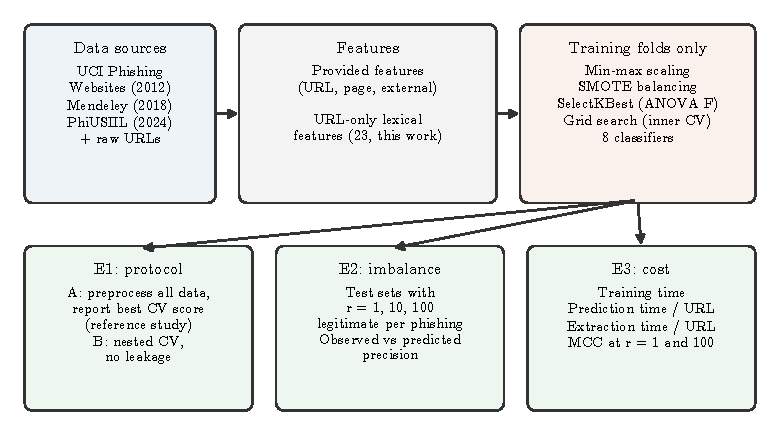
\includegraphics[width=0.95\textwidth]{fig_architecture.pdf}
\caption{Architecture of the evaluation framework. Scaling, SMOTE balancing, feature selection and hyper-parameter search are fitted on training folds only; the trained pipelines feed the three experiments}\label{fig:architecture}
\end{figure}

\subsection{Datasets}\label{subsec3-3}

Table~\ref{tab:datasets} lists the datasets. The UCI and Mendeley datasets are the two benchmarks of the reference study \cite{abdulsamad2023} and are used to replicate it in E1. PhiUSIIL \cite{prasad2024,prasad2024data} is used for E2 and E3 for three reasons: it is recent; it is more than twenty times larger than either benchmark, so test sets with 100 legitimate URLs per phishing URL can be drawn without reusing URLs; and it includes the raw URL string, so that lexical features can be computed independently of the supplied ones. Of its 54 features, the 50 numeric ones form the provided feature set; the remaining four (URL, domain, top-level domain and page title) are text. In every dataset the labels are recoded so that phishing is the positive class.

\begin{table}[htbp]
\caption{Datasets used in this study}\label{tab:datasets}%
\begin{tabular}{@{}lccccc@{}}
\toprule
Dataset & Year & Instances & Features & Phishing (\%) & Used in\\
\midrule
UCI \cite{mohammad2012uci} & 2012 & 11,055 & 30 & 44.3 & E1 \\
Mendeley \cite{tan2018} & 2018 & 10,000 & 48 & 50.0 & E1\footnotemark[1] \\
PhiUSIIL \cite{prasad2024,prasad2024data} & 2024 & 235,795 & 54\footnotemark[2] & 42.8 & E2, E3 \\
\botrule
\end{tabular}
\footnotetext{Class counts (legitimate / phishing): UCI 6,157 / 4,898; Mendeley 5,000 / 5,000; PhiUSIIL 134,850 / 100,945.}
\footnotetext[1]{Optional; requires a manual download.}
\footnotetext[2]{Plus the raw URL string, from which the lexical features of Table~\ref{tab:lexical} are computed.}
\end{table}

\subsection{URL-only lexical features}\label{subsec3-4}

A detector that runs when a user clicks a link must decide within milliseconds and, ideally, without visiting the suspicious page. The 23 features in Table~\ref{tab:lexical} meet both requirements: they are computed from the URL string with Python's standard URL parser, without downloading the page or contacting any external service. They describe length (of the URL, host, path and query), character counts (dots, hyphens, digits and special characters), structure (an IP address as host, an explicit port, the HTTPS scheme, sub-domains, path depth, query parameters, a double slash after the scheme and URL-shortening services), and two further signals: suspicious words such as \emph{login} or \emph{verify}, and the Shannon entropy of the characters. By contrast, eight of the 30 UCI features, including domain age, DNS record, web traffic, page rank and Google index, require external services, and most of the others require the page itself.

\begin{table}[htbp]
\caption{The 23 URL-only lexical features computed from the raw URL string}\label{tab:lexical}%
\begin{tabular}{@{}ll@{}}
\toprule
Feature & Description\\
\midrule
\texttt{url\_length} & Characters in the URL \\
\texttt{host\_length} & Characters in the host name \\
\texttt{path\_length} & Characters in the path \\
\texttt{query\_length} & Characters in the query string \\
\texttt{num\_dots} & Count of `.' \\
\texttt{num\_hyphens} & Count of `-' \\
\texttt{num\_underscores} & Count of `\_' \\
\texttt{num\_slashes} & Count of `/' \\
\texttt{num\_digits} & Count of digits \\
\texttt{digit\_ratio} & Digits divided by URL length \\
\texttt{num\_special} & Count of characters such as @ ? = \& \% \textasciitilde{} + \\
\texttt{has\_at} & URL contains `@' \\
\texttt{has\_ip\_host} & Host is an IPv4 or hexadecimal address \\
\texttt{is\_https} & Scheme is HTTPS \\
\texttt{num\_subdomains} & Host labels minus two \\
\texttt{has\_port} & An explicit port is given \\
\texttt{path\_depth} & Non-empty path segments \\
\texttt{double\_slash\_in\_path} & `//' appears after the scheme \\
\texttt{num\_params} & Query parameters \\
\texttt{tld\_length} & Length of the top-level domain \\
\texttt{is\_shortener} & Host is a known URL-shortening service \\
\texttt{suspicious\_words} & Words such as login, verify, account \\
\texttt{entropy} & Shannon entropy of the URL characters (bits) \\
\botrule
\end{tabular}
\end{table}

\subsection{Leakage-free training and tuning}\label{subsec3-5}

Algorithm~\ref{alg:nested} gives the leakage-free protocol, called protocol B. Each outer fold is held out once. On the remaining data, an inner cross-validation chooses the hyper-parameters and the number of selected features, and the chosen configuration is refitted on the whole outer training part before it is evaluated on the held-out fold, which is never resampled \cite{varma2006}. Scaling, SMOTE \cite{chawla2002} and feature selection are fitted only on training rows. To make this possible inside standard cross-validation tools, SMOTE is implemented as a wrapper around the classifier, so that it is applied at every fit and never to validation or test rows.

Protocol A reproduces the order of operations described by the reference study: the full dataset is min--max scaled and balanced with SMOTE, a grid search is then run with five-fold cross-validation on the balanced data, and the best cross-validated score is reported. Both protocols use the same classifiers, grids and folds of the original data, so the difference between them measures the combined effect of preprocessing before splitting and of reporting the tuning score itself. The reference study used ten-fold cross-validation; five folds are used here for both protocols to keep nested cross-validation affordable.

\begin{algorithm}
\caption{Leakage-free tuning and evaluation (protocol B)}\label{alg:nested}
\begin{algorithmic}[1]
\Require dataset $D$, classifier $c$, grid $G$, outer folds $K_o=5$, inner folds $K_i=3$
\Ensure mean and standard deviation of each metric over the outer folds
\For{each stratified outer split $(D_{\mathrm{tr}}, D_{\mathrm{te}})$ of $D$}
  \For{each configuration $g \in G$}
    \For{each stratified inner split $(T, V)$ of $D_{\mathrm{tr}}$}
      \State fit a min--max scaler on $T$ and apply it to $T$ and $V$
      \State $T' \gets \mathrm{SMOTE}(T)$ \Comment{synthetic rows built from $T$ only}
      \State remove constant columns; keep the $k_g$ best features of $T'$ by ANOVA $F$
      \State train $c$ with configuration $g$ on $T'$ and record its accuracy on $V$
    \EndFor
  \EndFor
  \State $g^\ast \gets$ the configuration with the highest mean inner accuracy
  \State refit the whole pipeline with $g^\ast$ on $D_{\mathrm{tr}}$
  \State compute accuracy, precision, recall, F1, MCC and PR-AUC on $D_{\mathrm{te}}$
\EndFor
\end{algorithmic}
\end{algorithm}

\subsection{Imbalance stress test}\label{subsec3-6}

Algorithm~\ref{alg:stress} describes E2. PhiUSIIL is split into a stratified 70\% training pool and a 30\% test pool. Each classifier is trained once, with default hyper-parameters and with scaling and SMOTE inside the pipeline, on a stratified sample of 20,000 rows of the training pool. Test sets are then drawn from the test pool with exactly $r$ legitimate URLs per phishing URL, for $r \in \{1, 10, 100\}$, and each draw is repeated ten times. The same draws are used for every classifier and feature set, so the comparisons are paired. The test pool holds 40,455 legitimate URLs, so the sets at $r=100$ contain 404 phishing URLs each.

\begin{algorithm}
\caption{Imbalance stress test (E2)}\label{alg:stress}
\begin{algorithmic}[1]
\Require trained pipeline $f$; held-out phishing set $P$ and legitimate set $L$; ratios $R=\{1,10,100\}$; repeats $n=10$
\Ensure mean and standard deviation of each metric per ratio; predicted precision per ratio
\For{each $r \in R$}
  \For{$j = 1, \dots, n$}
    \State $n_L \gets \min(|L|,\, r|P|)$; \quad $n_P \gets \lfloor n_L / r \rfloor$
    \State draw $n_P$ URLs from $P$ and $n_L$ URLs from $L$ without replacement
    \State compute accuracy, precision, recall, F1, MCC and PR-AUC of $f$ on the draw
  \EndFor
\EndFor
\State estimate $\mathrm{TPR}$ and $\mathrm{FPR}$ from the $r=1$ draws and predict precision with Eq.~(\ref{eq:prec-ratio})
\end{algorithmic}
\end{algorithm}

\subsection{Evaluation metrics}\label{subsec3-7}

Phishing is the positive class throughout, and $TP$, $FP$, $TN$ and $FN$ denote true and false positives and negatives. Eq.~(\ref{eq:basic}) defines precision, recall or true-positive rate (TPR) and false-positive rate (FPR); Eq.~(\ref{eq:f1}) combines precision and recall into the F1 score, and Eq.~(\ref{eq:mcc}) defines the MCC. Accuracy is reported for comparison with earlier work, but it says little under imbalance: at $r=100$ a classifier that labels every URL as legitimate is 99.0\% accurate and detects nothing. The MCC of Eq.~(\ref{eq:mcc}) is high only when all four cells of the confusion matrix are favourable \cite{chicco2020}, and the PR-AUC summarises the precision--recall trade-off, which is more informative than the ROC curve on imbalanced data \cite{saito2015}.

\begin{equation}
\mathrm{Precision} = \frac{TP}{TP+FP}, \qquad
\mathrm{TPR} = \mathrm{Recall} = \frac{TP}{TP+FN}, \qquad
\mathrm{FPR} = \frac{FP}{FP+TN}\label{eq:basic}
\end{equation}
\begin{equation}
F_1 = \frac{2\,\mathrm{Precision}\cdot\mathrm{Recall}}{\mathrm{Precision}+\mathrm{Recall}}\label{eq:f1}
\end{equation}
\begin{equation}
\mathrm{MCC} = \frac{TP\cdot TN - FP\cdot FN}{\sqrt{(TP+FP)(TP+FN)(TN+FP)(TN+FN)}}\label{eq:mcc}
\end{equation}
For a test set with $r$ legitimate URLs per phishing URL and fixed error rates,
\begin{equation}
\mathrm{Precision}(r) = \frac{\mathrm{TPR}}{\mathrm{TPR} + r\cdot\mathrm{FPR}},\label{eq:prec-ratio}
\end{equation}
and on a balanced test set ($r=1$) the false-positive rate follows from the reported precision $P$ and recall $R$ as
\begin{equation}
\mathrm{FPR} = R\left(\frac{1}{P}-1\right).\label{eq:fpr-balanced}
\end{equation}
Eq.~(\ref{eq:prec-ratio}) follows from Eq.~(\ref{eq:basic}): a test set with $N_P$ phishing and $rN_P$ legitimate URLs gives $TP=\mathrm{TPR}\cdot N_P$ and $FP=\mathrm{FPR}\cdot rN_P$. It assumes that the error rate on each class does not depend on the class ratio, which holds when the URLs of each class are drawn from the same distribution, as in E2. Eq.~(\ref{eq:fpr-balanced}) follows in the same way with $N_P=N_L=N$, $TP=RN$ and $FP=TP(1-P)/P$. It is used to obtain the false-positive rates implied by the results of the reference study in Fig.~\ref{fig:motivation}, and Eq.~(\ref{eq:prec-ratio}) is used to predict precision in E2.

\subsection{Use of AI tools}\label{subsec3-8}

In line with Springer Nature policy, the use of a large language model is reported here. Claude (Anthropic) was used, as permitted by the course instructor, to suggest the topic, search for and verify the literature, write the experiment code, run the experiments, and draft and format this manuscript. All numerical results were produced by running the published code on the public datasets, and no result was edited by hand. The author reviewed the manuscript and the code and takes full responsibility for the content.

%%=====================================================================%%
\section{Implementation and Experimental Setup}\label{sec4}

\subsection{Implementation}\label{subsec4-1}

The framework is written in Python using scikit-learn \cite{pedregosa2011} and XGBoost \cite{chen2016}. It is organised as a small package with one module per task: dataset loading, lexical feature extraction, SMOTE as a training-only wrapper, model and grid definitions, the three experiments, and plotting. A single script, \texttt{run\_experiments.py}, downloads the datasets, runs E1--E3, and writes the raw results as CSV files together with the tables and figures of Section~\ref{sec5}; a second script draws Figs.~\ref{fig:motivation} and \ref{fig:architecture}. Every random step uses the seed 42. The code, results and instructions are available at \url{https://github.com/nehatirkey-nsut/phishing-url-evaluation}.

\subsection{Experimental setup}\label{subsec4-2}

All experiments ran on an Apple M2 laptop with 8 CPU cores and 8\,GB of memory, using Python 3.13.3, scikit-learn 1.9.1, XGBoost 3.4.1, pandas 3.1.1 and NumPy 2.5.5. In E1, protocol B uses five stratified outer folds and three inner folds, and protocol A uses five-fold cross-validation; both search the grids in Table~\ref{tab:grid}, with the grid search parallelised over all cores. In E2 and E3, each classifier is trained single-threaded with its library-default hyper-parameters on 20,000 stratified rows of the PhiUSIIL training pool (165,056 URLs). The test pool holds 70,739 URLs, of which 40,455 are legitimate and 30,284 phishing, and each ratio is evaluated on ten random draws. Prediction time is measured on one batch of 10,000 test URLs and divided by the batch size, and lexical extraction time is measured over all 235,795 URLs. The complete run took about six minutes.

\begin{table}[htbp]
\caption{Hyper-parameter grids searched in E1 (all other settings are library defaults)}\label{tab:grid}%
\begin{tabular}{@{}lp{0.74\textwidth}@{}}
\toprule
Model & Values searched\\
\midrule
LogR & Logistic regression: $C \in \{0.01, 0.1, 1, 10, 100\}$ \\
SVM & Support vector machine, RBF kernel: $C \in \{1, 10\}$, $\gamma \in \{\text{scale}, 0.1\}$ \\
NB & Gaussian naive Bayes: variance smoothing $\in \{10^{-9}, 10^{-7}, 10^{-5}\}$ \\
KNN & $k$-nearest neighbours: $k \in \{3,5,7\}$, uniform or distance weights, Minkowski or Manhattan distance \\
DT & Decision tree: Gini or entropy, maximum depth $\in \{\text{none}, 20, 40\}$ \\
RF & Random forest, 200 trees: $\sqrt{d}$ or $\log_2 d$ features per split, depth $\in \{\text{none}, 40\}$ \\
GB & Gradient boosting: learning rate $\in \{0.1, 0.5\}$, trees $\in \{100, 300\}$ \\
XGB & XGBoost, 300 trees: depth $\in \{6, 12\}$, learning rate $\in \{0.1, 0.3\}$ \\
All & SelectKBest with ANOVA $F$: $k \in \{10, 20, \text{all}\}$ features \\
\botrule
\end{tabular}
\end{table}

%%=====================================================================%%
\section{Results}\label{sec5}

\subsection{E1: effect of the evaluation protocol}\label{subsec5-1}

Tables~\ref{tab:e1-uci} and \ref{tab:e1-mendeley} list the E1 results and Fig.~\ref{fig:e1} shows the difference between the two protocols. Protocol A reproduces the reference study closely. On UCI, seven of the eight classifiers come within 0.73 percentage points of the reported accuracy; for example, random forest reaches 97.48\% against 97.44\% reported, and gradient boosting 97.34\% against 97.47\%. The exception is naive Bayes (78.44\% against 91.27\%), because this study uses the Gaussian variant while the reference study used the Bernoulli variant on UCI.

Under the leakage-free protocol B, every classifier scores lower on UCI than under protocol A: by 0.25 to 0.65 points for seven classifiers and by 2.73 points for naive Bayes, with a mean of 0.43 points when naive Bayes is excluded. The direction is the same for all eight classifiers; if the sign of each difference were random, eight positive differences would occur with a probability of 0.008 (two-sided sign test). Individually, the differences are comparable to the fold-to-fold standard deviations of protocol B (0.11 to 0.48 points for the seven classifiers), so it is their consistent direction, more than their size, that makes them noteworthy. The best leakage-free results on UCI are 97.11 $\pm$ 0.34\% for XGBoost and 97.04 $\pm$ 0.25\% for random forest, while gradient boosting, the best model of the reference study, reaches 96.70 $\pm$ 0.11\%, which is 0.77 points below its reported accuracy.

On the Mendeley dataset, which is already balanced and therefore not resampled, the two protocols agree within 0.26 points (mean 0.06), and two classifiers (random forest and XGBoost) even score marginally higher under protocol B. Since the main difference between the protocols on Mendeley is the absence of oversampling before the split, this contrast indicates that most of the gap observed on UCI comes from applying SMOTE to the full dataset, rather than from reporting the tuning score. Leakage-free accuracy on Mendeley reaches 98.87 $\pm$ 0.19\% with XGBoost, above the 98.21\% reported for that model. Under protocol B the MCC ranges from 0.850 to 0.941 on UCI and from 0.890 to 0.977 on Mendeley for all classifiers except naive Bayes.

\begin{table}[htbp]
\caption{E1 results on the UCI dataset: accuracy (\%) reported by the reference study, obtained with its protocol (A) and with leakage-free nested cross-validation (B, mean $\pm$ s.d.\ over five outer folds), their difference, and the MCC under protocol B}\label{tab:e1-uci}%
\begin{tabular}{@{}lcccrc@{}}
\toprule
Model & Reported & Protocol A & Protocol B & A $-$ B & MCC (B) \\
\midrule
LogR & 92.33 & 92.82 & 92.57 $\pm$ 0.28 & $+0.25$ & 0.850 \\
SVM & 97.04 & 96.31 & 95.91 $\pm$ 0.15 & $+0.40$ & 0.917 \\
NB & 91.27 & 78.44 & 75.71 $\pm$ 1.21 & $+2.73$ & 0.598 \\
KNN & 97.04 & 96.96 & 96.45 $\pm$ 0.36 & $+0.52$ & 0.928 \\
DT & 96.69 & 96.65 & 96.39 $\pm$ 0.48 & $+0.26$ & 0.927 \\
RF & 97.44 & 97.48 & 97.04 $\pm$ 0.25 & $+0.44$ & 0.940 \\
GB & 97.47 & 97.34 & 96.70 $\pm$ 0.11 & $+0.65$ & 0.933 \\
XGB & 97.26 & 97.58 & 97.11 $\pm$ 0.34 & $+0.47$ & 0.941 \\
\botrule
\end{tabular}
\end{table}

\begin{table}[htbp]
\caption{E1 results on the Mendeley dataset: accuracy (\%) reported by the reference study, obtained with its protocol (A) and with leakage-free nested cross-validation (B, mean $\pm$ s.d.\ over five outer folds), their difference, and the MCC under protocol B}\label{tab:e1-mendeley}%
\begin{tabular}{@{}lcccrc@{}}
\toprule
Model & Reported & Protocol A & Protocol B & A $-$ B & MCC (B) \\
\midrule
LogR & 93.88 & 94.49 & 94.48 $\pm$ 0.45 & $+0.01$ & 0.890 \\
SVM & 96.79 & 97.05 & 97.02 $\pm$ 0.59 & $+0.03$ & 0.940 \\
NB & 86.99 & 84.62 & 84.62 $\pm$ 0.95 & $+0.00$ & 0.707 \\
KNN & 95.41 & 95.75 & 95.49 $\pm$ 0.21 & $+0.26$ & 0.910 \\
DT & 96.17 & 97.04 & 96.90 $\pm$ 0.33 & $+0.14$ & 0.938 \\
RF & 97.79 & 98.33 & 98.34 $\pm$ 0.17 & $-0.01$ & 0.967 \\
GB & 98.27 & 98.50 & 98.39 $\pm$ 0.57 & $+0.11$ & 0.968 \\
XGB & 98.21 & 98.83 & 98.87 $\pm$ 0.19 & $-0.04$ & 0.977 \\
\botrule
\end{tabular}
\end{table}

\begin{figure}[htbp]
\centering
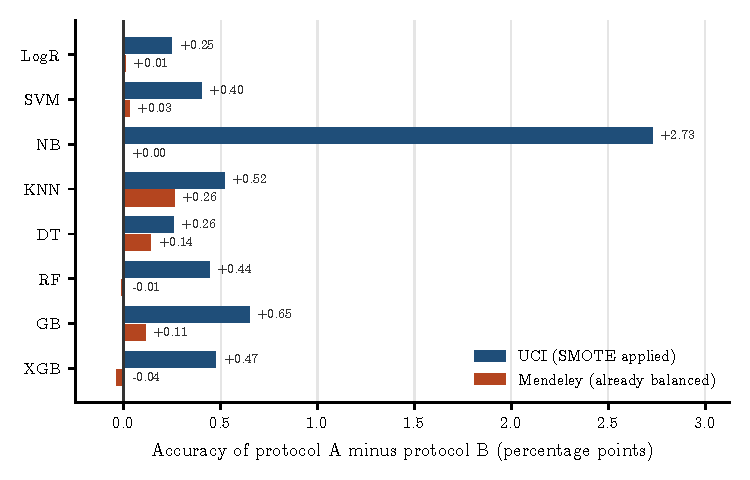
\includegraphics[width=0.95\textwidth]{fig_e1_protocols.pdf}
\caption{Difference in accuracy between the reference protocol (A), which scales and SMOTE-balances the whole dataset before cross-validation, and leakage-free nested cross-validation (B), for each classifier. SMOTE is applied to UCI only, because the Mendeley dataset is already balanced}\label{fig:e1}
\end{figure}

\subsection{E2: effect of class imbalance}\label{subsec5-2}

Tables~\ref{tab:e2-provided} and \ref{tab:e2-lexical} and Fig.~\ref{fig:e2} show the E2 results, which follow three patterns. First, recall does not change with the class ratio (for example, 91.7 to 91.8\% for logistic regression with lexical features), which confirms the assumption behind Eq.~(\ref{eq:prec-ratio}). The precision predicted from the $r=1$ error rates matches the observed precision within 0.47 points in all 48 combinations of feature set, classifier and ratio, with a mean absolute difference of 0.04 points.

Second, with the features supplied with PhiUSIIL the task is almost trivial. The decision tree, random forest, gradient boosting and XGBoost make no false positives on any of the 40,455 legitimate test URLs, so their precision remains 100\% at $r=100$. Logistic regression, the support vector machine and naive Bayes fall only to 98.1\%, 99.5\% and 95.3\%. The exception is $k$-nearest neighbours, whose false-positive rate of 0.55\% reduces its precision to 64.1\%.

Third, with URL-only lexical features every classifier still exceeds 99.18\% precision on balanced test sets, but at $r=100$ precision ranges from 54.9\% for logistic regression, whose false-positive rate is 0.75\%, to 99.2\% for the support vector machine, whose false-positive rate is 0.007\%. In between lie gradient boosting (95.2\%), random forest (86.9\%), XGBoost (82.4\%), the decision tree (69.3\%), naive Bayes (63.4\%) and $k$-nearest neighbours (63.2\%). Accuracy hides this decline: for logistic regression it rises from 95.48\% at $r=1$ to 99.17\% at $r=100$, while precision falls from 99.18\% to 54.86\% and the MCC from 0.912 to 0.706.

\begin{table}[htbp]
\caption{E2 results on PhiUSIIL with provided features: observed precision (\%, mean $\pm$ s.d.\ over repeated draws), precision predicted from the $r=1$ error rates, recall (\%), MCC and PR-AUC (\%) at each ratio $r$ of legitimate to phishing URLs}\label{tab:e2-provided}%
\begin{tabular}{@{}lrccccc@{}}
\toprule
Model & $r$ & Precision & Predicted & Recall & MCC & PR-AUC \\
\midrule
LogR & 1 & 100.0 $\pm$ 0.0 & 100.0 & 99.8 & 0.998 & 100.0 \\
 & 10 & 99.8 $\pm$ 0.0 & 99.8 & 99.9 & 0.998 & 100.0 \\
 & 100 & 98.1 $\pm$ 0.0 & 98.1 & 99.8 & 0.989 & 99.9 \\
SVM & 1 & 100.0 $\pm$ 0.0 & 100.0 & 99.9 & 0.999 & 100.0 \\
 & 10 & 100.0 $\pm$ 0.0 & 99.9 & 99.9 & 0.999 & 100.0 \\
 & 100 & 99.5 $\pm$ 0.0 & 99.4 & 99.9 & 0.997 & 100.0 \\
NB & 1 & 100.0 $\pm$ 0.0 & 100.0 & 100.0 & 0.999 & 100.0 \\
 & 10 & 99.5 $\pm$ 0.0 & 99.5 & 100.0 & 0.997 & 99.7 \\
 & 100 & 95.3 $\pm$ 0.0 & 95.2 & 100.0 & 0.976 & 97.3 \\
KNN & 1 & 99.4 $\pm$ 0.0 & 99.4 & 99.0 & 0.985 & 99.7 \\
 & 10 & 94.7 $\pm$ 0.0 & 94.6 & 99.0 & 0.965 & 98.4 \\
 & 100 & 64.1 $\pm$ 0.1 & 63.7 & 99.1 & 0.795 & 88.4 \\
DT & 1 & 100.0 $\pm$ 0.0 & 100.0 & 100.0 & 1.000 & 100.0 \\
 & 10 & 100.0 $\pm$ 0.0 & 100.0 & 100.0 & 1.000 & 100.0 \\
 & 100 & 100.0 $\pm$ 0.0 & 100.0 & 100.0 & 1.000 & 100.0 \\
RF & 1 & 100.0 $\pm$ 0.0 & 100.0 & 100.0 & 1.000 & 100.0 \\
 & 10 & 100.0 $\pm$ 0.0 & 100.0 & 100.0 & 1.000 & 100.0 \\
 & 100 & 100.0 $\pm$ 0.0 & 100.0 & 100.0 & 1.000 & 100.0 \\
GB & 1 & 100.0 $\pm$ 0.0 & 100.0 & 100.0 & 1.000 & 100.0 \\
 & 10 & 100.0 $\pm$ 0.0 & 100.0 & 100.0 & 1.000 & 100.0 \\
 & 100 & 100.0 $\pm$ 0.0 & 100.0 & 100.0 & 1.000 & 100.0 \\
XGB & 1 & 100.0 $\pm$ 0.0 & 100.0 & 100.0 & 1.000 & 100.0 \\
 & 10 & 100.0 $\pm$ 0.0 & 100.0 & 100.0 & 1.000 & 100.0 \\
 & 100 & 100.0 $\pm$ 0.0 & 100.0 & 99.9 & 1.000 & 100.0 \\
\botrule
\end{tabular}
\end{table}

\begin{table}[htbp]
\caption{E2 results on PhiUSIIL with URL-only lexical features: observed precision (\%, mean $\pm$ s.d.\ over repeated draws), precision predicted from the $r=1$ error rates, recall (\%), MCC and PR-AUC (\%) at each ratio $r$ of legitimate to phishing URLs}\label{tab:e2-lexical}%
\begin{tabular}{@{}lrccccc@{}}
\toprule
Model & $r$ & Precision & Predicted & Recall & MCC & PR-AUC \\
\midrule
LogR & 1 & 99.2 $\pm$ 0.0 & 99.2 & 91.7 & 0.912 & 99.4 \\
 & 10 & 92.4 $\pm$ 0.0 & 92.4 & 91.8 & 0.913 & 97.2 \\
 & 100 & 54.9 $\pm$ 0.4 & 54.9 & 91.8 & 0.706 & 91.9 \\
SVM & 1 & 100.0 $\pm$ 0.0 & 100.0 & 98.2 & 0.982 & 99.8 \\
 & 10 & 99.9 $\pm$ 0.0 & 99.9 & 98.2 & 0.990 & 99.6 \\
 & 100 & 99.2 $\pm$ 0.0 & 99.2 & 98.0 & 0.986 & 99.0 \\
NB & 1 & 99.4 $\pm$ 0.0 & 99.4 & 98.5 & 0.979 & 99.4 \\
 & 10 & 94.6 $\pm$ 0.0 & 94.6 & 98.5 & 0.962 & 95.3 \\
 & 100 & 63.4 $\pm$ 0.1 & 63.5 & 98.2 & 0.787 & 68.7 \\
KNN & 1 & 99.4 $\pm$ 0.0 & 99.4 & 98.2 & 0.976 & 99.4 \\
 & 10 & 94.5 $\pm$ 0.0 & 94.4 & 98.2 & 0.960 & 97.8 \\
 & 100 & 63.2 $\pm$ 0.1 & 62.8 & 97.9 & 0.784 & 87.1 \\
DT & 1 & 99.6 $\pm$ 0.0 & 99.6 & 99.0 & 0.986 & 99.1 \\
 & 10 & 95.8 $\pm$ 0.0 & 95.8 & 99.0 & 0.971 & 95.0 \\
 & 100 & 69.3 $\pm$ 0.1 & 69.7 & 98.8 & 0.825 & 68.5 \\
RF & 1 & 99.9 $\pm$ 0.0 & 99.9 & 99.1 & 0.989 & 99.8 \\
 & 10 & 98.5 $\pm$ 0.0 & 98.5 & 99.1 & 0.987 & 99.5 \\
 & 100 & 86.9 $\pm$ 0.0 & 87.0 & 98.9 & 0.926 & 99.0 \\
GB & 1 & 100.0 $\pm$ 0.0 & 100.0 & 98.9 & 0.989 & 99.7 \\
 & 10 & 99.5 $\pm$ 0.0 & 99.5 & 98.9 & 0.991 & 98.6 \\
 & 100 & 95.2 $\pm$ 0.0 & 95.3 & 98.8 & 0.970 & 92.3 \\
XGB & 1 & 99.8 $\pm$ 0.0 & 99.8 & 98.9 & 0.987 & 99.8 \\
 & 10 & 97.9 $\pm$ 0.0 & 97.9 & 99.0 & 0.983 & 99.4 \\
 & 100 & 82.4 $\pm$ 0.1 & 82.4 & 98.8 & 0.902 & 98.8 \\
\botrule
\end{tabular}
\end{table}

\begin{figure}[htbp]
\centering
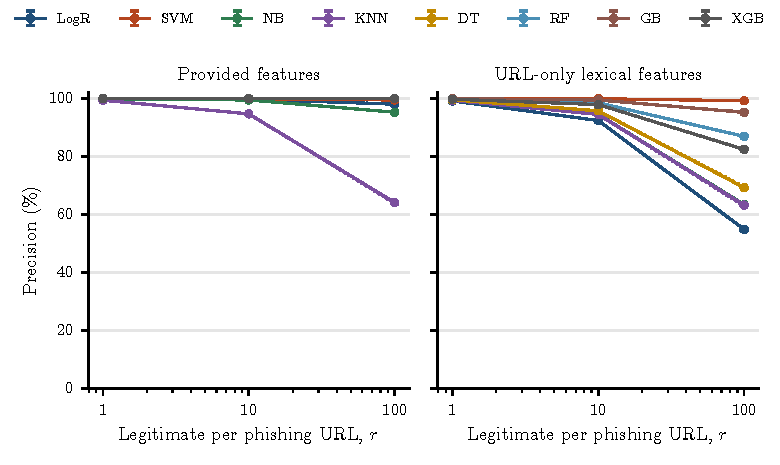
\includegraphics[width=0.95\textwidth]{fig_e2_imbalance.pdf}
\caption{Observed precision (solid, mean $\pm$ s.d.\ over 10 draws) and precision predicted by Eq.~(\ref{eq:prec-ratio}) from the $r=1$ error rates (dotted) as the ratio of legitimate to phishing URLs grows}\label{fig:e2}
\end{figure}

\subsection{E3: computational cost and URL-only features}\label{subsec5-3}

Table~\ref{tab:e3} shows that none of the classifiers is expensive. Training on 20,000 URLs takes at most 2.8\,s (gradient boosting with the provided features). Prediction takes at most 68\,$\mu$s per URL (the support vector machine with lexical features), and below 10\,$\mu$s for every classifier except the support vector machine and $k$-nearest neighbours. Extracting the 23 lexical features takes 11.8\,$\mu$s per URL in plain Python, so a complete URL-only decision with gradient boosting takes about 13\,$\mu$s on a single core. The provided features, by contrast, include page-level counts such as lines of code, images, scripts and references, which can only be obtained by downloading and parsing the page. Their cost depends on network access and was not measured.

The price of URL-only features is a lower MCC: from 0.912 to 0.989 at $r=1$ and from 0.706 to 0.986 at $r=100$, against 0.985 to 1.000 and 0.795 to 1.000 with the provided features. Among the lexical models, the support vector machine keeps the highest precision at $r=100$ (99.2\%, MCC 0.986) but is the slowest, while gradient boosting reaches an MCC of 0.970 at $r=100$ with a prediction time of 1.0\,$\mu$s per URL.

\begin{table}[htbp]
\caption{E3 results on PhiUSIIL: training time, prediction and lexical-feature extraction time per URL, and MCC at $r=1$ and $r=100$ for the provided features (Prov., 50 features) and the URL-only lexical features (Lex., 23 features)}\label{tab:e3}%
\begin{tabular}{@{}llrrrrr@{}}
\toprule
Feat. & Model & Train (s) & Pred.\ ($\mu$s) & Extr.\ ($\mu$s) & MCC$_{r=1}$ & MCC$_{r=100}$ \\
\midrule
Prov. & LogR & 0.2 & 0.5 & -- & 0.998 & 0.989 \\
Prov. & SVM & 0.3 & 15.6 & -- & 0.999 & 0.997 \\
Prov. & NB & 0.1 & 0.5 & -- & 0.999 & 0.976 \\
Prov. & KNN & 0.1 & 16.1 & -- & 0.985 & 0.795 \\
Prov. & DT & 0.1 & 0.5 & -- & 1.000 & 1.000 \\
Prov. & RF & 1.9 & 4.3 & -- & 1.000 & 1.000 \\
Prov. & GB & 2.8 & 1.0 & -- & 1.000 & 1.000 \\
Prov. & XGB & 0.4 & 1.2 & -- & 1.000 & 1.000 \\
Lex. & LogR & 0.1 & 0.3 & 11.8 & 0.912 & 0.706 \\
Lex. & SVM & 1.2 & 67.9 & 11.8 & 0.982 & 0.986 \\
Lex. & NB & 0.1 & 0.4 & 11.8 & 0.979 & 0.787 \\
Lex. & KNN & 0.0 & 10.3 & 11.8 & 0.976 & 0.784 \\
Lex. & DT & 0.1 & 0.3 & 11.8 & 0.986 & 0.825 \\
Lex. & RF & 1.1 & 9.3 & 11.8 & 0.989 & 0.926 \\
Lex. & GB & 1.4 & 1.0 & 11.8 & 0.989 & 0.970 \\
Lex. & XGB & 0.4 & 2.2 & 11.8 & 0.987 & 0.902 \\
\botrule
\end{tabular}
\end{table}

\subsection{Why PhiUSIIL is easy to classify}\label{subsec5-feat}

The near-perfect scores with the provided features call for an explanation. Table~\ref{tab:features} reports how well each feature separates the classes on its own, using a classifier with a single threshold. The \texttt{URLSimilarityIndex} feature alone classifies 99.66\% of URLs correctly, and four page-content counts each exceed 94\%, so the supplied feature set leaves little to learn. The raw URLs show a second, simpler artefact: every legitimate URL in the dataset is an HTTPS home page with no path (not even a trailing slash) and no query string, whereas 32.7\% of phishing URLs end in a single slash, 27.2\% have a longer path and 51.3\% do not use HTTPS. A lexical model can therefore score well by recognising the form of a home-page URL, which explains why the length of the path and the HTTPS indicator are the strongest single lexical features.

\begin{table}[htbp]
\caption{Accuracy of a single-threshold classifier (one-split decision tree, 5-fold cross-validation on 50,000 PhiUSIIL URLs) for the strongest individual features of each set}\label{tab:features}%
\begin{tabular}{@{}llr@{}}
\toprule
Feature set & Feature & Accuracy (\%) \\
\midrule
Provided & \texttt{URLSimilarityIndex} & 99.66 \\
Provided & \texttt{NoOfExternalRef} & 96.09 \\
Provided & \texttt{LineOfCode} & 95.56 \\
Provided & \texttt{NoOfSelfRef} & 94.74 \\
Provided & \texttt{NoOfImage} & 94.18 \\
Lexical & \texttt{path\_length} & 82.74 \\
Lexical & \texttt{num\_slashes} & 82.74 \\
Lexical & \texttt{is\_https} & 79.13 \\
\botrule
\end{tabular}
\footnotetext{In the full dataset, 100.0\% of legitimate URLs have no path (not even a trailing slash), 0.0\% have a query string and 100.0\% use HTTPS; for phishing URLs the shares are 40.1\%, 6.0\% and 48.7\%, and 32.7\% end in a single slash.}
\end{table}

\subsection{Comparison with existing approaches}\label{subsec5-4}

Table~\ref{tab:compare} places the best results of this study beside the strongest earlier results on the same datasets. Under the reference protocol, XGBoost reaches 97.58\% on UCI, slightly above every earlier result; under leakage-free evaluation it reaches 97.11\%, below all three. The position of a method in this ranking therefore depends on the evaluation protocol as much as on the method. On Mendeley, leakage-free XGBoost (98.87\%) is above both earlier results, which agrees with the finding of E1 that the protocol matters little on balanced data. Because the earlier studies differ in folds, grids and preprocessing, which are not always fully reported, these comparisons are indicative rather than exact.

\begin{table}[htbp]
\caption{Comparison with the strongest earlier results on the same datasets (accuracy, \%)}\label{tab:compare}%
\begin{tabular}{@{}llll@{}}
\toprule
Dataset & Study & Method & Accuracy\\
\midrule
UCI & Salihovic et al.\ \cite{salihovic2019} & RF + Ranker + PCA & 97.33 \\
 & Al-Sarem et al.\ \cite{alsarem2021} & Optimised stacking ensemble & 97.16 \\
 & Abdul Samad et al.\ \cite{abdulsamad2023} & Tuned gradient boosting & 97.47 \\
 & This work, protocol A & XGBoost & 97.58 \\
 & This work, protocol B & XGBoost & 97.11 $\pm$ 0.34 \\
\midrule
Mendeley & Al-Sarem et al.\ \cite{alsarem2021} & Optimised stacking ensemble & 98.58 \\
 & Abdul Samad et al.\ \cite{abdulsamad2023} & Tuned gradient boosting & 98.27 \\
 & This work, protocol A & XGBoost & 98.83 \\
 & This work, protocol B & XGBoost & 98.87 $\pm$ 0.19 \\
\botrule
\end{tabular}
\end{table}

%%=====================================================================%%
\section{Discussion}\label{sec6}

The answer to RQ1 is that preprocessing the whole dataset before cross-validation does inflate accuracy, modestly but consistently: by about half a percentage point for the strong classifiers on UCI, and not measurably on the balanced Mendeley data, where no oversampling takes place. Half a point sounds small, but it is as large as the differences that separate the best published methods in Table~\ref{tab:prior}. Rankings at the top of these benchmarks can therefore reflect the protocol rather than the model. The remedy costs little: resampling and scaling belong inside the cross-validation loop, and accuracy should be estimated with nested cross-validation \cite{varma2006}.

The answer to RQ2 is that precision under class imbalance is governed by the false-positive rate, and that it can be predicted almost exactly from results on balanced data with Eq.~(\ref{eq:prec-ratio}). A detector with a false-positive rate of 0.75\% loses almost half of its alarms to false positives when legitimate URLs outnumber phishing URLs 100 to 1, even though its accuracy rises above 99\%. Since the prediction needs only the true- and false-positive rates, every study can report the precision implied at realistic ratios at no extra cost, together with the MCC and PR-AUC \cite{saito2015,chicco2020}.

The answer to RQ3 is that model choice is not limited by computation: every classifier trains in seconds and predicts in microseconds. The real cost lies in obtaining the features. URL-only features cost about 12\,$\mu$s per URL and still give an MCC of 0.97 at $r=100$ with gradient boosting, whereas the supplied page-level features need the page to be downloaded. Their near-perfect scores, however, mostly reflect how PhiUSIIL was built: a single feature almost separates the classes, and all legitimate URLs are home pages. The URL-only results are optimistic for the same reason, because the lexical models can recognise the form of a home-page URL.

These findings have practical consequences. A detector that is deployed, whether in a browser or as a cloud service such as PhishNot \cite{alani2022}, sees mostly legitimate traffic, so its usefulness depends on keeping the false-positive rate far below 1\%, not on a further gain in balanced accuracy. Benchmark datasets would serve this goal better if their legitimate class contained ordinary deep links rather than only home pages, and if they were split by collection date, because phishing changes over time \cite{gama2014}. Representation-learning models \cite{le2018,elsadig2022} report high accuracy as well, and they should be evaluated under the same leakage-free, imbalance-aware protocol before they are compared with feature-based models.

Several limitations apply. E1 uses five folds instead of the ten of the reference study, smaller grids and the Gaussian rather than the Bernoulli variant of naive Bayes, so its protocol A is a close but not exact replication. E2 and E3 use default hyper-parameters, a single training sample of 20,000 URLs and a single random seed. The repeated test draws reuse the same pool of legitimate URLs, so their standard deviations understate how much results would vary across datasets. Timings were measured on one laptop with single-threaded Python and will differ on other hardware. Finally, the artefacts of PhiUSIIL limit how far the E2 and E3 results generalise; an independent, recent dataset whose legitimate class includes deep links is needed to confirm them.

%%=====================================================================%%
\section{Conclusion and Future Work}\label{sec7}

This study re-examined the 97--98\% accuracies reported for fine-tuned phishing URL classifiers with three experiments. Replicating the reference study showed that balancing the whole dataset before cross-validation inflated the accuracy of all eight classifiers on the UCI dataset, by 0.25 to 2.73 percentage points, while the balanced Mendeley dataset showed no such effect; leakage-free XGBoost reached 97.11\% on UCI and 98.87\% on Mendeley. A stress test on 235,795 recent URLs showed that the precision of URL-only detectors falls to between 54.9\% and 99.2\% when legitimate URLs outnumber phishing URLs 100 to 1, as predicted within 0.5 points by a simple formula, while accuracy rises. All models were fast enough for real-time use, and the 23 URL-only features took 12\,$\mu$s per URL to compute; but the near-perfect scores obtained with PhiUSIIL's own features reflect how the dataset was built rather than a solved problem.

Benchmark accuracy therefore overstates how well phishing detectors would work in practice. Future work should evaluate detectors on datasets whose legitimate URLs include deep links and are split by collection date, test models across datasets, compare grid search with more efficient Bayesian optimisation \cite{akiba2019}, and evaluate character-level deep models \cite{le2018} under the same leakage-free, imbalance-aware protocol.

%%=====================================================================%%
\backmatter

\bmhead{Supplementary information}

Not applicable.

\bmhead{Acknowledgements}

Not applicable.

\section*{Declarations}

\begin{itemize}
\item Funding: No funding was received for this work.
\item Conflict of interest/Competing interests: The author declares no competing interests.
\item Ethics approval and consent to participate: Not applicable.
\item Consent for publication: Not applicable.
\item Data availability: The datasets analysed in this study are publicly available: UCI Phishing Websites \cite{mohammad2012uci}, Mendeley phishing dataset \cite{tan2018} and PhiUSIIL \cite{prasad2024data}.
\item Materials availability: Not applicable.
\item Code availability: The source code, results and figures are available at \url{https://github.com/nehatirkey-nsut/phishing-url-evaluation}.
\item Author contribution: The author reviewed and approved the code, the results and the manuscript, which were prepared with the AI assistance described in Section~\ref{subsec3-8}.
\end{itemize}

\bibliography{sn-bibliography}

\end{document}
